% Pitch deck for the Feyer "Faster Physics" challenge, START Hack Munich 2026.
% Build: cd docs/pitch && pdflatex pitch.tex && pdflatex pitch.tex
% Every number comes from results/amd-epyc-final/comparison.txt (AMD EPYC 9334, 1 CPU, one session).
\documentclass[aspectratio=169,11pt]{beamer}

\usepackage[utf8]{inputenc}
\usepackage[T1]{fontenc}
\usepackage{lmodern}
\usepackage{amsmath,amssymb}
\usepackage{booktabs}
\usepackage{adjustbox}
\usepackage{tikz}
\usetikzlibrary{arrows.meta,positioning}

\graphicspath{{../report/figures/}}

% ---------------------------------------------------------------- look
\definecolor{accent}{HTML}{C0262D}   % red accent
\definecolor{ink}{HTML}{222222}
\definecolor{muted}{HTML}{6B7280}
\definecolor{good}{HTML}{009E73}
\definecolor{panel}{HTML}{F3F4F6}

\usefonttheme{professionalfonts}
\setbeamertemplate{navigation symbols}{}
\setbeamercolor{normal text}{fg=ink}
\setbeamercolor{frametitle}{fg=accent}
\setbeamercolor{title}{fg=ink}
\setbeamercolor{subtitle}{fg=muted}
\setbeamercolor{structure}{fg=accent}
\setbeamercolor{itemize item}{fg=accent}
\setbeamerfont{frametitle}{series=\bfseries,size=\Large}
\setbeamerfont{title}{series=\bfseries,size=\huge}
\setbeamertemplate{itemize items}[circle]
\setbeamertemplate{footline}{%
  \hspace{1.2em}\color{muted}\scriptsize Feyer $\cdot$ Faster Physics \hfill \insertframenumber\,/\,\inserttotalframenumber\hspace{1.2em}\vspace{0.8em}}

\newcommand{\bignum}[1]{{\fontsize{40}{44}\selectfont\bfseries #1}}
\newcommand{\hl}[1]{\textcolor{accent}{\textbf{#1}}}
\newcommand{\ok}[1]{\textcolor{good}{\textbf{#1}}}
\newcommand{\src}[1]{\par\vfill{\color{muted}\scriptsize Source: #1}}

% Fill in before presenting.
\newcommand{\team}{Team name}

\title{Differometor, 60$\times$ faster}
\subtitle{Same physics, same gradients: 35.3\,s $\to$ 0.585\,s for the complete first run}
\author{\team}
\institute{START Hack Munich 2026 $\cdot$ Feyer: Faster Physics}
\date{22 November 2026}

\begin{document}

% ================================================================= 1
\begin{frame}[plain]
  \titlepage
\end{frame}

% ================================================================= 2
\begin{frame}{The result}
  \centering
  \vspace{0.4em}
  \begin{columns}[T]
    \begin{column}{0.32\textwidth}\centering
      {\color{muted}complete first run (scored)}\\[0.3em]
      \bignum{0.585\,s}\\[0.2em]
      \hl{60$\times$} \;{\color{muted}from 35.28\,s}
    \end{column}
    \begin{column}{0.32\textwidth}\centering
      {\color{muted}warm evaluation}\\[0.3em]
      \bignum{0.081\,s}\\[0.2em]
      \hl{190$\times$} \;{\color{muted}from 15.48\,s}
    \end{column}
    \begin{column}{0.32\textwidth}\centering
      {\color{muted}XLA compilation}\\[0.3em]
      \bignum{0.17\,s}\\[0.2em]
      \hl{112$\times$} \;{\color{muted}from 19.23\,s}
    \end{column}
  \end{columns}
  \vspace{1.6em}
  \begin{itemize}
    \item All 101 frequencies, all 193 design variables, \texttt{float64}/\texttt{complex128}, no precomputation.
    \item \ok{21 of 21 runs PASS.} $\max|\Delta\log S| = 5.374\times10^{-6}$: the same error as the unmodified code.
    \item One session, one pinned core of an AMD EPYC 9334: baseline and every variant side by side.
  \end{itemize}
  \src{results/amd-epyc-final/comparison.txt (median of 3 runs; spread $<2\%$)}
\end{frame}

% ================================================================= 3
\begin{frame}{Where the 35 seconds went}
  \begin{columns}[c]
    \begin{column}{0.48\textwidth}
      \begin{tabular}{@{}lr@{}}
        \toprule
        Baseline phase & seconds \\
        \midrule
        Imports \& setup & 0.97 \\
        \hl{XLA trace / lower / compile} & \hl{19.23} \\
        Forward simulation & 12.14 \\
        Gradient & 2.94 \\
        \midrule
        \textbf{Complete first run} & \textbf{35.28} \\
        \bottomrule
      \end{tabular}
    \end{column}
    \begin{column}{0.5\textwidth}
      \begin{itemize}
        \item Over half the time is \hl{compiling}: a 19-way \texttt{lax.switch} per component, dense assembly and its reverse pass.
        \item The rest is \hl{dense linear algebra} on a $751\times751$ system that is \textbf{99.55\,\% zeros}.
        \item 6 dense solves per frequency $\times$ 101 frequencies = \textbf{606} LU factorisations.
      \end{itemize}
    \end{column}
  \end{columns}
  \src{results/amd-epyc-final/baseline\_\{1,2,3\}.json}
\end{frame}

% ================================================================= 4
\begin{frame}{Idea 1: stop storing zeros, factorise once}
  \centering
  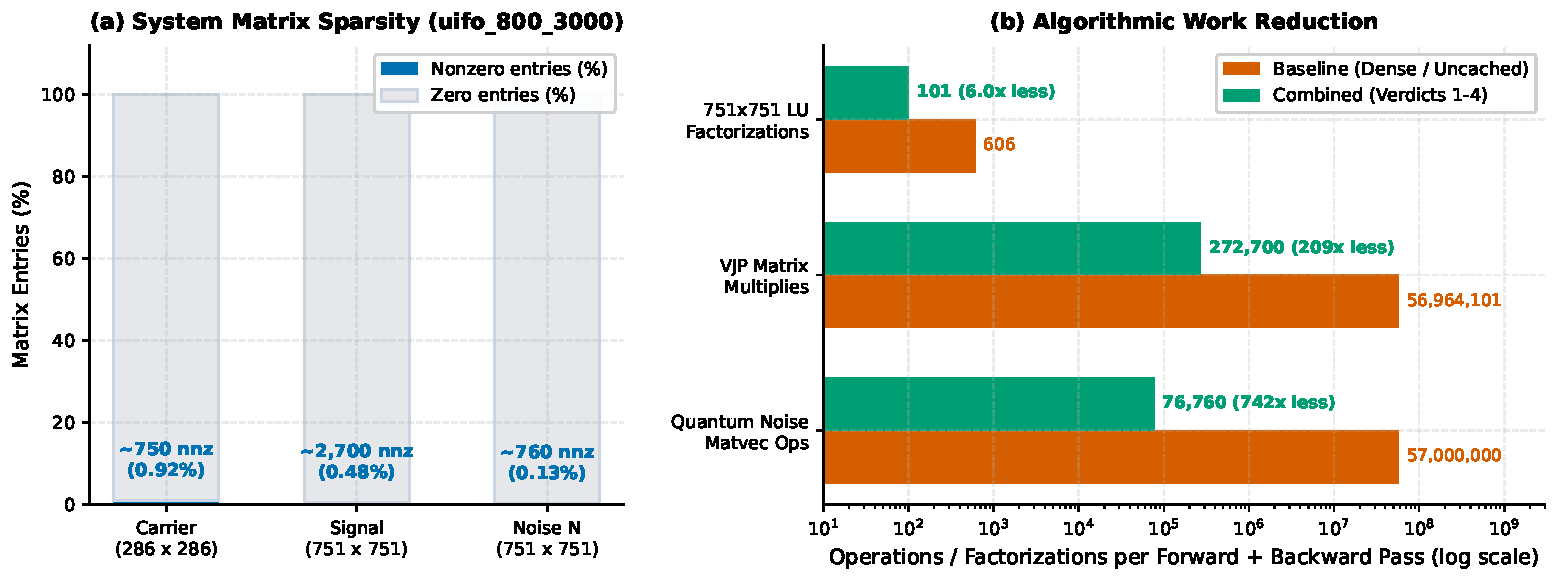
\includegraphics[width=\linewidth,height=0.5\textheight,keepaspectratio]{fig1_matrix_sparsity_and_work.pdf}
  \begin{columns}[T]
    \begin{column}{0.48\textwidth}
      \begin{itemize}
        \item Signal matrix: \textbf{2,537} nonzeros of 564,001; noise: 272.
        \item Compressed assembly: every write position mapped once at build time.
      \end{itemize}
    \end{column}
    \begin{column}{0.5\textwidth}
      \begin{itemize}
        \item \hl{One LU per frequency}, reused for $Ax=b$, $A^Hw=c$ and both adjoint solves: 606 $\to$ \textbf{101}.
        \item Sparse VJP $\bar v_e = -\lambda_{r_e}x_{c_e}$ only at nonzeros: \textbf{222$\times$} fewer operations.
      \end{itemize}
    \end{column}
  \end{columns}
\end{frame}

% ================================================================= 5
\begin{frame}{Idea 2: one identity deletes a whole solve}
  Quantum noise needs $\;\operatorname{Re}\big(c^H A^{-1} N A^{-H} c\big)$. The original code solved twice:
  \[
    w = A^{-H}c, \qquad v = A^{-1}(N w), \qquad \text{noise} = \operatorname{Re}(c^H v).
  \]
  But $c^H A^{-1} = (A^{-H}c)^H = w^H$, so
  \[
    \boxed{\;\text{noise} = \operatorname{Re}\big(w^H N w\big)\;}
  \]
  \begin{itemize}
    \item Exact for every invertible $A$ and any $N$: valid for every topology, not just this one.
    \item $N$ does not depend on frequency $\Rightarrow$ evaluated once, contracted over its 272 nonzeros (\textbf{2,074$\times$} fewer operations).
  \end{itemize}
\end{frame}

% ================================================================= 6
\begin{frame}{Idea 3: run the physics on the host, keep JAX's derivatives}
  \begin{columns}[c]
    \begin{column}{0.5\textwidth}
      \begin{itemize}
        \item The whole simulation runs in NumPy/C++ inside \hl{one \texttt{jax.custom\_vjp}}: XLA compiles two tiny callback stubs instead of the assembly graph.
        \item Component physics is \emph{not} re-derived by hand: JAX's own JVP program is \hl{transposed} into the VJP (matches \texttt{jax.vjp} to $\le 2.7\times10^{-16}$).
        \item 19 closed-form \hl{Wirtinger-dual kernels} skip tracing entirely; custom components fall back automatically.
      \end{itemize}
    \end{column}
    \begin{column}{0.48\textwidth}
      \centering
      \begin{tabular}{@{}lrr@{}}
        \toprule
        & baseline & ours \\
        \midrule
        forward compile & 12.67\,s & 0.009\,s \\
        gradient compile & 4.62\,s & 0.034\,s \\
        forward run & 12.14\,s & 0.047\,s \\
        \bottomrule
      \end{tabular}\\[0.8em]
      {\small\color{muted} \texttt{DIFFEROMETOR\_BACKEND=jax} keeps the full in-graph path (forward-mode AD, Hessians).}
    \end{column}
  \end{columns}
  \src{first-run phase medians, results/amd-epyc-final/comparison.txt}
\end{frame}

% ================================================================= 7
\begin{frame}{Idea 4: our own sparse LU in C++}
  \begin{itemize}
    \item Gilbert--Peierls left-looking LU (CSparse/KLU style), loaded with \texttt{ctypes}, compiled at \texttt{pip install}.
    \item Minimum-degree ordering on $A+A^T$, computed once per sparsity pattern.
    \item \hl{KLU-style pivot reuse}: frequency 0 is pivoted; the other 100 reuse its pivot order whenever every pivot stays $\ge 0.1\times$ the column maximum. On the benchmark, all 100 reuse it.
    \item One step of iterative refinement on every solve; a singular frequency gives \texttt{NaN} only for itself.
  \end{itemize}
  \vspace{0.6em}
  \begin{block}{What we rejected, and why}
    COLAMD-style ordering ($A^TA$): 30\,\% less fill, but a $10^{-2}$ log error on Voyager space modulation. The tiny solution components the noise form depends on are ordering-sensitive. Accuracy won.
  \end{block}
\end{frame}

% ================================================================= 8
\begin{frame}{Idea 5: the last 70 ms, without changing a single bit}
  After ideas 1--4, the biggest phase we could still change was \hl{compiling the benchmark's own readout} (234 HLO lines, yet 0.13\,s).
  \vspace{0.4em}
  \begin{columns}[T]
    \begin{column}{0.5\textwidth}
      \textbf{E11: cheaper XLA code generation}
      \begin{itemize}
        \item The cost is per fusion, not per graph size.
        \item The package selects XLA's classic emitters before the backend starts.
        \item Compile 0.238 $\to$ \textbf{0.171\,s}; outputs \ok{bit-identical}.
      \end{itemize}
    \end{column}
    \begin{column}{0.5\textwidth}
      \textbf{E12: CPU-tuned solver, same rounding}
      \begin{itemize}
        \item \texttt{-march=native} for wider SIMD\ldots
        \item \ldots with \texttt{-ffp-contract=off}: no fused multiply-add, so every operation rounds as before.
        \item Factorisation $-17\,\%$; \ok{bit-identical} on 12 topologies.
      \end{itemize}
    \end{column}
  \end{columns}
  \vspace{0.6em}
  {\small Opt-in \texttt{DIFFEROMETOR\_XLA\_FLAGS=fast}: \textbf{0.509\,s (69$\times$)}, at the cost of one sensitivity moving by 1\,ulp.}
\end{frame}

% ================================================================= 9
\begin{frame}{Every variant, one session}
  \centering
  % panels (b) and (c) of the report's figure 2: the scored first run, and a zoom on the optimised variants
  \adjincludegraphics[width=\linewidth,height=0.66\textheight,keepaspectratio,trim={{0.355\width} 0 0 0},clip]{fig2_benchmark_comparison.pdf}\\[0.3em]
  {\small Baseline $\to$ team milestones $\to$ committed v2 (0.656\,s) $\to$ final \textbf{0.585\,s}. Same machine, same core, interleaved runs.}
  \src{results/amd-epyc-final/ (3 runs $\times$ 10 warm repeats per variant)}
\end{frame}

% ================================================================= 10
\begin{frame}{Correct, and in places more accurate than the original}
  \begin{columns}[T]
    \begin{column}{0.5\textwidth}
      \textbf{Benchmark checks (all 21 runs)}
      \begin{itemize}
        \item $\max|\Delta\log S| = 5.374\times10^{-6}$ (bar $10^{-5}$); identical to the unmodified code.
        \item Gradient vs.\ baseline: cosine \textbf{1.0000000000}, relative error $8.6\times10^{-8}$.
        \item Finite-difference check: error $4.3\times10^{-9}$, against $7.0\times10^{-8}$ for the original code.
        \item Also checked on aLIGO, Voyager, UIFO and random topologies.
      \end{itemize}
    \end{column}
    \begin{column}{0.48\textwidth}
      \textbf{Against 50-digit references}\\[0.3em]
      \small
      \begin{tabular}{@{}lrr@{}}
        \toprule
        log error & dense & ours \\
        \midrule
        UIFO 3$\times$3, seed 1 & $1.1\times10^{-3}$ & $2.2\times10^{-10}$ \\
        Voyager AM & $1.8\times10^{-4}$ & $2.2\times10^{-6}$ \\
        \bottomrule
      \end{tabular}\\[0.5em]
      {\small Sparse LU with iterative refinement beats dense LAPACK on ill-conditioned setups ($\kappa \sim 10^{31}$).}
    \end{column}
  \end{columns}
  \src{results/amd-epyc-final/, results/generality-e9.jsonl, tests/}
\end{frame}

% ================================================================= 11
\begin{frame}{What we learned}
  \begin{itemize}
    \item \hl{Compile time was the real enemy}, not FLOPs: 19\,s of 35\,s. The fastest code is the code XLA never sees.
    \item \hl{Structure beats hardware}: sparsity, one identity and pivot reuse gave more than any amount of tuning.
    \item \hl{Measure every phase}: the last 70\,ms came from a 234-line program nobody would have suspected.
    \item \hl{Bit-identical is achievable}: it made every speed-up provable, not just ``close enough''.
  \end{itemize}
  \vspace{0.8em}
  \textbf{What is left:} \texttt{import jax} alone is 0.26\,s of our 0.585\,s. Next: vectorise the LU across frequencies (same pivot order $\Rightarrow$ SIMD over 101 systems, still bit-identical).
\end{frame}

% ================================================================= 12
\begin{frame}[fragile]{Reproduce it}
\begin{verbatim}
pip install -r requirements.txt && pip install -e .
python benchmark.py --cpus 1 --output final.json   # prints PASS
DIFFEROMETOR_XLA_FLAGS=fast python benchmark.py --cpus 1
\end{verbatim}
  \vspace{0.4em}
  \begin{itemize}
    \item Fallbacks: \texttt{DIFFEROMETOR\_NATIVE=0} (SciPy SuperLU), \texttt{DIFFEROMETOR\_BACKEND=jax} (in-graph JAX).
    \item Write-ups: \texttt{OPTIMIZATION\_LOG.md}, \texttt{docs/report/main.pdf}, \texttt{docs/notes/}.
  \end{itemize}
  \vspace{1.2em}
  \centering
  {\Large\bfseries 35.28\,s $\;\longrightarrow\;$ \textcolor{accent}{0.585\,s}}\par\vspace{0.3em}
  {\color{muted}Thank you. Questions?}\par
\end{frame}

\end{document}
